\section{Implementation of Networks}
\label{sec:implementation_networks}

\subsection{Overview}

In chapter \ref{chapter:xbrl} we introduced the concept of networks,
followed by Brel's interpretation of networks in chapter \ref{chapter:api}.
% We also looked at the different types of networks that are defined in the XBRL 2.1 specification.
% In this chapter, we will look at how networks are represented in XBRL and how Brel parses them.
% As previously mentioned, one of the main goals of Brel is to shield the user from the complexity of the XBRL specification.
% Brel achieves this on two different levels.
% First, Brel provides a simple API that allows users to access and traverse networks independent of the type of network.
% This API provides methods for traversing any directed acyclic graph.
% It is intended for advanced users and is useful for debugging networks in a report.
% For example, for each network, Brel provides a function that returns all direct children of a node in the network.
% Second, Brel implements a wrapper around each type of network.
% This wrapper provides a clean interface for some of the most common operations on networks.
% The functionality of the wrapper depends on the type of network.
% For example, the wrapper for calculation networks provides functions to validate the calculation network and to calculate the value of a concept.
% We will first look at the common interface for all networks.
% Then, we will look at the different types of networks and see how they diverge from the common interface.
% \subsection{Common Interface}
A network in Brel comprises of two different classes: \texttt{INetwork} and \texttt{INetworkNode}.
% Python does not support interfaces, so we used abstract base classes to define the interface of networks in Brel.

A network in Brel is a directed acyclic graph.
\footnote{The XBRL specification does allow cycles in networks, but Brel does not support them.}
Each node in the graph has an ordered list of children and at most one parent.
The network does not necessarily have to be connected, i.e. there can be multiple disconnected subgraphs in the network.

Technically speaking, a network in Brel is just a set of root nodes.
These nodes point to their children, which in turn point to their children, and so on.
So, to traverse a network, we only need to know the root nodes of the network.
The \texttt{INetwork} class provides a method to get all root nodes of the network
and the \texttt{INetworkNode} class provides a method to get all children of a node,
which allows us to traverse the network.

One implementation detail of networks in Brel is that they cannot be empty.
They have to contain at least one node.
The functionality of an "empty" network can still be achieved by letting the component of the network point to \texttt{None}.

% The following UML diagram shows the class diagram of the \texttt{INetwork} class. 
% The classes \texttt{QName}, \texttt{IReportElement}, \texttt{IResource}, and \texttt{Fact} are depicted in a simplified form.

% \begin{figure}[H]
%     \caption{Class diagram of the \texttt{INetwork} and \texttt{INetworkNode} classes}
%     \label{fig:inetwork_class_diagram}
%     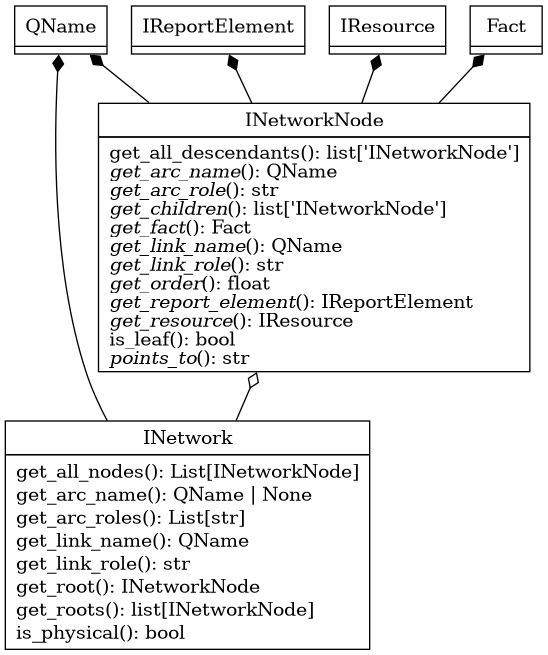
\includegraphics[width=0.8\textwidth]{images/i_networks_uml.png}
% \end{figure}

% First, we will look at the methods of the \texttt{INetwork} class.

% \subsubsection{INetwork}

% The \texttt{INetwork} class provides the following methods:

% \begin{itemize}
%     \item \texttt{get\_roots}: Returns a list of all root nodes of the network.
%     \item \texttt{get\_root}: Returns the root node of the network if the network has exactly one root node, otherwise it raises an exception.
%     \item \texttt{get\_all\_nodes}: Returns a list of all nodes that are part of the network i.e. all nodes that are reachable from the root nodes.
%     \item \texttt{get\_link\_role}: Returns the link role of the network. 
%     The link role is usually the URI of the component that the network belongs to.
%     If the network does not belong to a component, it returns the standard link role \texttt{http://www.xbrl.org/2003/role/link}.
%     \item \texttt{get\_link\_name}: Returns the link QName of the network.
%     This can be \texttt{link:presentationLink}, \texttt{link:calculationLink}, etc.
%     \item \texttt{get\_arc\_roles}: Returns all the different arc roles that are used by nodes in the network.
%     For most networks, this will only be one arc role.
%     For example, for a calculation network, this will be \texttt{summation-item}.
%     However, for a definition network, multiple arc roles can be used within the same network.
%     \item \texttt{get\_arc\_name}: Returns the arc QName of all arcs in the network.
%     All arcs in the network must have the same arc name.
%     For example, for a calculation network, this will be \texttt{link:calculationArc}.
%     Since a network can consist of a single node, it is possible that the network does not contain any arcs.
%     In that case, the method returns \texttt{None}.
%     \item \texttt{is\_physical}: Returns \texttt{True} if the network is a physical network, otherwise it returns \texttt{False}.
%     For all physical networks, the whole network can only have a single arc role.
% \end{itemize}

% \subsubsection{INetworkNode}

% The \texttt{INetworkNode} class provides the following methods:

% \begin{itemize}
%     \item \texttt{get\_children}: Returns a list of all direct children of the node.
%     The children are sorted by their order attribute.
%     \item \texttt{get\_get\_all\_descendants}: Returns a list of the transitive closure of the children of the node.
%     \item \texttt{get\_order}: Returns the order attribute of the node.
%     \item \texttt{is\_leaf}: Returns \texttt{True} if the node has no children, otherwise it returns \texttt{False}.
%     \item \texttt{get\_link\_role}: Returns the link role of the network that the node belongs to.
%     \item \texttt{get\_link\_name}: Returns the link QName of the network that the node belongs to.
%     \item \texttt{get\_arc\_role}: Returns the arc role of the arc that connects the node to its parent.
%     \item \texttt{get\_arc\_name}: Returns the arc QName of the arc that connects the node to its parent.
%     \item \texttt{points\_to}: Returns the type of element that the node points to.
%     This can either be 'report element', 'resource' or 'fact'.
%     \item \texttt{get\_report\_element}: Returns the report element that the node points to.
%     Raises an exception if the node does not point to a report element.
%     \item \texttt{get\_resource}: Returns the resource that the node points to.
%     Raises an exception if the node does not point to a resource.
%     \item \texttt{get\_fact}: Returns the fact that the node points to.
%     Raises an exception if the node does not point to a fact.

% \end{itemize}

% Given these two interfaces, we can now discuss how Brel parses links into networks.

\subsection{Parsing Links into Networks}

Section \ref{sec:xbrl_networks} introduced the different types of networks, and how they are all just a collection of arcs, locators and resources.
It also explained how locators and resources represent nodes and how arcs represent edges in a network.
So parsing a link into a network is just a matter of converting a list of nodes and edges into a graph.
Brel's algorithm for parsing links consists of four steps:

\begin{enumerate}\label{enum:network_parsing}
    \item First, it iterates over all elements of the link. 
    If the element is a locator or a resource, it creates an instance of the \texttt{INetworkNode} class.
    If the element is an arc, Brel stores the from and to attributes of the arc in an edge list.
    \item For the second step, Brel can assume that all nodes have been created.
    So, it iterates over the edge list and adds adds the to-node as a child to the from-node.
    \item Next, Brel iterates over all nodes and adds all nodes that do not have a parent to the root list of the network.
    The root list is then wrapped into a \texttt{INetwork} instance.
    \item Finally, if the network has any implications on the report as a whole, Brel will apply these implications to the report.
    For example, if the label network adds a label to a concept, Brel will add the label to the concept in the report.
    The exact implications depend on the type of network.
\end{enumerate}

% So far, we have only looked at the common interface of networks.
% In reality, there are different types of networks that have different functionality.
Chapter \ref{chapter:api} introduced the different types of networks.
For each type of network, Brel provides both a node class and a network class, 
all of which inherit from the \texttt{INetwork} and \texttt{INetworkNode} classes respectively.
% There exists a factory method for each type of network or node that returns the correct network or node class for the given link.
Brel uses the factory pattern to create the correct network and node instances for a given link.
Each type of network has its own factory.
The factories are used by the algorithm \ref{enum:network_parsing} to create the correct network and node instances.

\subsection{Resolving Locators}

As mentioned in section \ref{sec:xbrl_networks}, locators are used to point to report elements or facts.
This section will explain how Brel resolves locators.

XBRL locators use XPointer\cite{w3_xpointer} expressions to reference other XML elements, which are potentially defined in other XML documents.
The XPointers XBRL uses are of the form \texttt{filename\#id},
where \texttt{filename} is the name of the XML document and \texttt{id} is the id of the XML element.
% XPointers use the "id" attribute of XML elements to reference them.
% So, to resolve a locator, Brel first needs to find the XML element that the locator points to.
To resolve a locator, Brel first needs to find the XML element that the locator points to.
Then, it needs to resolve the XML element into a report element or a fact.

Brel does this by remembering the id of each fact and report element that it has parsed.
It builds a lookup table that maps ids to facts and report elements.
Whenever Brel encounters a locator during the parsing process, it resolves the locator by looking up the id of the locator in the lookup table.
% It builds a dictionary that maps ids to facts and report elements.
% Then, when it encounters a locator, it uses the id of the locator to look up the fact or report element that the locator points to.

\subsection{Parsing Resources}

Resources are the other type of element that can be referenced by arcs.
Unlike locators, resources are not used to point to other elements in the report.
Instead, they directly contain the value of the element that they represent.

The current specification of XBRL 2.1 defines three built-in types of resources: label, reference and footnote.
Custom resources are also possible.

Resources consist of three elements: a role, a label and a value.

The role is a URI that identifies the type of resource.
For example, the role \texttt{http://www.xbrl.org/2003/role/terseLabel} identifies a label resource that contains a short label for a concept, 
whereas the role \texttt{http://www.xbrl.org/2003/role/footnote} identifies a footnote resource that contains a footnote for a concept.

The label acts as an identifier for the resource.
The label is used by arcs to reference the resource.
Do not confuse the label of a resource with a human readable label for a concept.

The value of a resource contains the actual resource.
For labels, the value is the text of the label.
For references, this is the dictionary that points to some exteral resource like an article in the SEC's Code of Federal Regulations.

Since resources have all the information that is needed to parse them, Brel does not need to resolve any references to parse them.
Therefore, parsing them is very straightforward.

\subsection{Implications of Networks}

As mentioned in section \ref{enum:network_parsing}, networks can have implications on the report as a whole.
There are two implications that are common to all networks: Labels and LineItems promoting.

\subsection{Add Labels to Report Elements}

Labels are used to provide human-readable names for report elements.
They are created using the label network \texttt{link:labelLink}.
Labellinks are described in more detail in section \ref{sec:labelLink}.
Brel parses report elements before it parses networks, since many networks contain locators that point to report elements.
So, when Brel parses a label network, it already knows all report elements that are referenced by the locators in the network.

Once the label network has been parsed, Brel iterates over all labels in the network.
It then adds the label to the report element that the locator of the label points to.

\subsection{LineItems Promoting}

Report elements are defined in the taxonomy and there six different types: concepts, abstracts, lineitems, members, dimensions and hypercubes.
When looking at an XML element in the taxonomy, it is not always clear what type of report element it represents.
Both abstracts and lineitems are represented by a structurally identical XML element.
There are two approaches to tell them apart: 

\begin{enumerate}
    \item The first approach is to look at the QName of the element.
    Lineitems often have the substring "LineItems" in their QName.
    The problem with this approach is that this is more of a convention than a rule.
    There is no guarantee that the QName of a lineitem will contain the substring "LineItems".
    \item The second approach is to look at how the element is used in networks.
    specifically, definition networks define the relationships between report elements.
    The arc role \texttt{hypercube-dimension} is used to define the relationship between a hypercube report element and a dimension report element.
    Similarly, the arc role \texttt{all} is used to define the relationship between a hypercube report element and a lineitem report element.
\end{enumerate}

Brel uses the second approach to tell lineitems and abstracts apart.
Initially, Brel assumes that all report elements are abstracts.
Then, when it parses a definition network, it looks at the arc roles of the arcs in the network.
If the network contains an arc with the arc role \texttt{all} and the arc lies between a hypercube and an abstract, Brel assumes that the abstract is a lineitem.


This concludes the chapter on the implementation of networks.
Together with previous sections of this chapter, it covered all parts of XBRL and how Brel parses them.
However, section \ref{sec:implementation_report_elements} made a key assumption about taxonomies that is not always true.
% It assumed that all taxonomies agree on how each 
Each taxonomy can import other taxonomies under a prefix-URI pair.
The assumption was that all taxonomies agree on the prefix-URI pair of each taxonomy.
This assumption is not always true.
The next section will explain how Brel handles this situation. 